\section{Everything that was run}
\label{app:experiments}

Sixteen sweeps, 582 episodes, 2{,}328 beats, one model family except where noted. This
appendix is the complete record: what each sweep varied, what it establishes, and the two
that establish nothing. Numbers are recomputed from per-episode summaries over delivered
beats, with percentile bootstrap intervals; \S\ref{sec:quantifying} states why delivery is
tabulated before any contrast.

\begin{table}[h]
\centering\small
\caption{Every sweep. ``ep'' is episodes; each episode is four beats.}
\label{tab:allruns}
\begin{tabular}{@{}p{0.14\linewidth}p{0.26\linewidth}r p{0.40\linewidth}@{}}
\toprule
\textbf{Sweep} & \textbf{Varied} & \textbf{ep} & \textbf{What it establishes} \\
\midrule
\texttt{realistic}   & $2\times2$ $\times$ $E$          & 72  & Main decomposition: $0.232 / 0.080 / \approx\!0$ \\
\texttt{axis2x2}     & $2\times2$ $\times$ $E$          & 72  & Independent replication of the same \\
\texttt{matched-E0}  & three arms, $E=0$                & 27  & \textbf{Zero-dose control: the gap disappears} \\
\texttt{main}        & three arms $\times$ $E$          & 54  & Read-all $\approx$ open; public $-$ private $=+0.240$ \\
\texttt{matched-E0-glm} & second model, $E=0$           & 18  & The control replicates; the main effect is untested \\
\texttt{scaling}     & edge cost $\times$ relay depth   & 112 & Brokered hop $+0.140$; per-edge cost is null \\
\texttt{seedaxis}    & six attribute profiles           & 72  & Attribute axis flat; placebo $+0.005$ \\
\texttt{repscan}     & reputation off/real/random       & 48  & Null, but the design is at fault (\S\ref{app:reputation}) \\
\texttt{capscan}     & search cap 5/20/80               & 24  & Reading 16$\times$ more results buys nothing \\
\texttt{nscan}       & directory 50--800                & 60  & \textbf{Retracted} (\S\ref{app:retracted}) \\
\texttt{k-pilot}     & deliverable complexity           & 8   & Pilot only \\
five smoke sweeps    & mechanism checks                 & 15  & Confirm each manipulation fires \\
\bottomrule
\end{tabular}
\end{table}

\subsection{Formation: the dose-response and its control}
\label{app:dose}

\metric{E} is the share of required facts placed outside the roster.

\begin{center}\small
\begin{tabular}{@{}lrrrlrr@{}}
\toprule
\textbf{$E$} & \textbf{open} & \textbf{bounded} & \textbf{$\Delta$} & \textbf{95\% CI} & \textbf{bounded sources} & \textbf{bounded fabrications} \\
\midrule
$0.0$ & 0.823 & 0.789 & $+0.034$ & $[-0.067, +0.137]$ spans 0 & 4.36 & 0.000 \\
$0.3$ & 0.791 & 0.679 & $+0.111$ & $[+0.020, +0.200]$ & 3.17 & 0.139 \\
$0.7$ & 0.803 & 0.524 & $+0.279$ & $[+0.210, +0.345]$ & 1.26 & 0.333 \\
\bottomrule
\end{tabular}
\end{center}

Four properties hold together, and the paper's use of this axis rests on all four: the
zero-dose contrast spans zero; the arm that should be unaffected is flat
($0.823/0.791/0.803$); the mechanism variable tracks the dose; and the failure mode
appears only as sources dry up. The $E=0$ cells come from the three-arm generation of
the harness (\texttt{matched-E0}), which is why they are reported alongside rather than
inside the $2\times2$.

\subsection{The credulity result}
\label{app:credulity}

Pooled over \texttt{realistic} and \texttt{axis2x2}, restricted to delivered beats
(287 open, 286 bounded):

\begin{center}\small
\begin{tabular}{@{}lrrl@{}}
\toprule
& \textbf{open} & \textbf{bounded} & \textbf{difference} \\
\midrule
misinformation shown           & $\sim4\times$ more & baseline & the roster is genuinely cleaner \\
absorbed into the deliverable  & 0.094 / task & 0.269 / task & $+0.175$\quad CI $[+0.105, +0.242]$ \\
fabricated outright            & 1 instance   & 58 instances & --- \\
\bottomrule
\end{tabular}
\end{center}

\metric{absorbed} requires that the agent was shown the distractor; \metric{fabricated}
requires that it was not, so the second is a value invented that happens to coincide with
a planted wrong one---a conservative lower bound on fabrication, since only coincidences
with planted values are detectable. Stratifying by the number of useful sources obtained
does not remove the gap: at four useful sources the absorption rate is 2.4\% open against
18.1\% bounded, so starvation amplifies the effect but is not the whole of it.

\subsection{Introduction against endorsement}
\label{app:relay2}

From \texttt{scaling}, arm C, relay depth 0 against 1, balanced across all three edge-cost
levels (28 episodes each):

\begin{center}\small
\begin{tabular}{@{}lrrrr@{}}
\toprule
\textbf{Architecture} & \textbf{$F_1$} & \textbf{useful sources} & \textbf{absorption} & \textbf{fabrications/task} \\
\midrule
bounded, island            & 0.553 & 1.50 & 11.0\% & 0.223 \\
bounded, one brokered hop  & 0.693 & 3.40 & 6.3\%  & 0.057 \\
read-all, deep only inside & 0.836 & --- & --- & 0.000 \\
open                       & 0.857 & 4.63 & 2.4\%  & 0.000 \\
\bottomrule
\end{tabular}
\end{center}

The hop is worth $+0.140$ (CI $[+0.073, +0.204]$) conditional on delivery and $+0.088$
(CI $[+0.016, +0.158]$) with lost beats scored as zero, and it clears zero independently
within each edge-cost stratum ($+0.128$, $+0.138$, $+0.173$). Read-all against open is
$+0.019$ and spans zero. This supersedes an earlier estimate of $+0.042$ (CI
$[-0.137, +0.208]$) computed from a 16-episode cell; the number in Table~\ref{tab:allruns}
is the 28-per-arm one.

\subsection{Nulls worth reporting}

\paragraph{Per-edge cost does not move the ranking.} Charging a handshake turn for each
contact outside the roster---194 and 384 handshakes fired at costs of one and two
turns---leaves the open arm's advantage at $+0.219$, $+0.263$, $+0.244$ across the three
levels while its tokens rise from 53k to 74k. The arm absorbs friction as cost rather
than as failure. An earlier draft named this as the variable most likely to reverse the
ranking and stated it had not been run; both halves of that sentence are corrected here.

\paragraph{Reading more search results buys nothing.} Caps of 5, 20 and 80 give
$0.791$, $0.755$, $0.819$, every contrast spanning zero.

\paragraph{Attributes.} Six profiles against a length-matched placebo; see
\S\ref{app:seeds} for the seed texts and \S\ref{sec:evidence} for the numbers.

\subsection{Reputation: a null caused by the task, not the mechanism}
\label{app:reputation}

Marks were differential---counterparts that held a planted falsehood were flagged, and a
random-mark arm held the wording fixed while removing the information. All three arms are
identical: $0.821$ off, $0.817$ real, $0.833$ random, every contrast spanning zero.

The design is at fault. Each fact has exactly one holder, so a flagged counterpart is
also the only route to the true values it holds; a requester that avoided flagged cards
would lose more than it gained, and routing measurement confirms it moved \emph{toward}
them. Making the mark actionable requires two holders per fact, one reliable and one not,
which is a change to fact allocation rather than to the reputation mechanism. We report
this as a failed manipulation rather than as evidence about reputation.

\subsection{The retracted directory-size sweep}
\label{app:retracted}

\texttt{nscan} varied the directory from 50 to 800 cards and appeared to show the open
arm's advantage decaying to zero. It does not. 27\% of its beats produced no artifact,
every one of them ending in a transport failure after four retries, and the scorer's
$F_1=0$ for a beat with no artifact was averaged in as a score. Other sweeps lost 2--3\%.

\begin{figure}[t]
\centering
\definecolor{openarm}{HTML}{2A78D6}
\definecolor{bndarm}{HTML}{C4551F}
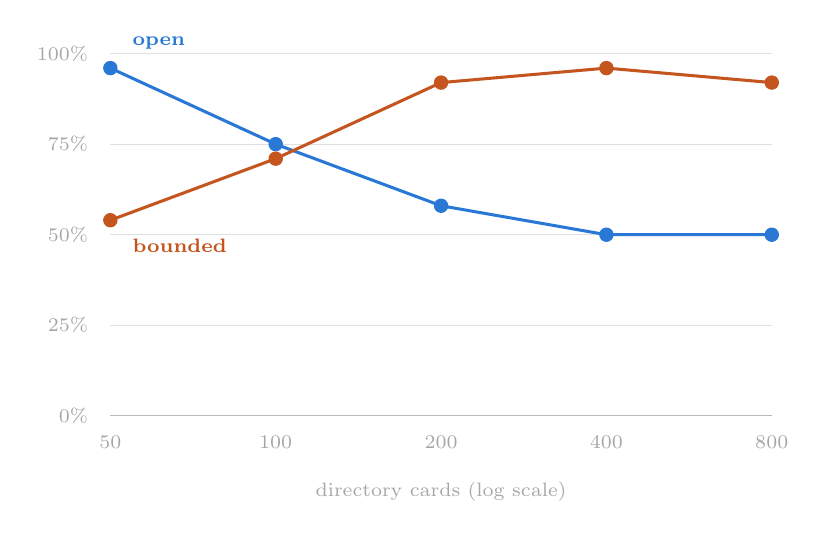
\begin{tikzpicture}[x=1.05cm,y=1.15cm,font=\small]
  % grid and axes
  \foreach \y/\l in {0/0\%, 1/25\%, 2/50\%, 3/75\%, 4/100\%} {
    \draw[gray!25] (0,\y) -- (8,\y);
    \node[anchor=east,gray!70,font=\scriptsize] at (-0.15,\y) {\l};
  }
  \draw[gray!55] (0,0) -- (8,0);
  \foreach \x/\l in {0/50, 2/100, 4/200, 6/400, 8/800}
    \node[anchor=north,gray!70,font=\scriptsize] at (\x,-0.12) {\l};
  \node[anchor=north,gray!70,font=\scriptsize] at (4,-0.62) {directory cards (log scale)};

  % open arm: delivery falls
  \draw[openarm,line width=1.1pt] (0,3.84) -- (2,3.00) -- (4,2.32) -- (6,2.00) -- (8,2.00);
  \foreach \x/\y in {0/3.84, 2/3.00, 4/2.32, 6/2.00, 8/2.00}
    \filldraw[openarm] (\x,\y) circle (2.4pt);
  \node[openarm,anchor=south west,font=\scriptsize\bfseries] at (0.15,3.94) {open};

  % bounded arm: delivery rises -- and it never sees more than twenty cards
  \draw[bndarm,line width=1.1pt] (0,2.16) -- (2,2.84) -- (4,3.68) -- (6,3.84) -- (8,3.68);
  \foreach \x/\y in {0/2.16, 2/2.84, 4/3.68, 6/3.84, 8/3.68}
    \filldraw[bndarm] (\x,\y) circle (2.4pt);
  \node[bndarm,anchor=north west,font=\scriptsize\bfseries] at (0.15,2.06) {bounded};
\end{tikzpicture}
\caption{Delivery rate in the retracted sweep: the share of episodes that produced an
artifact at all. \textcolor{openarm}{\textbf{The open arm}} falls with directory size and
\textcolor{bndarm}{\textbf{the bounded arm}} rises. The bounded arm reads a twenty-card
roster at every setting, so directory size is not in its causal path and its delivery rate
cannot be responding to it. Both curves are the same transport outage, sampled by two arms
that happened to walk their size settings in opposite orders. Scoring the missing artifacts
as $F_1 = 0$ turned this figure into a scaling result.}
\label{fig:delivery}
\end{figure}

Three checks establish that the losses are not caused by directory size. The bounded arm
reads a twenty-card roster at every setting, so size is not in its causal path, yet its
delivery rate rose from 54\% to 96\% across the sweep (Figure~\ref{fig:delivery}). Scenario was collinear with wall
clock---one scenario ran entirely inside the failure window---and the two arms walked
their size settings in opposite orders inside it, which is what drew one line down and the
other up. And lost beats used 4.4 of 22+ available turns with zero build calls while
taking \emph{longer} in wall clock, which is a stalled connection rather than an exhausted
budget.

Conditional on delivery both arms are flat: the open arm runs $0.800, 0.777, 0.758,
0.779, 0.826$ across a 16$\times$ range ($\Delta = -0.026$, CI $[-0.123, +0.065]$). In the
one cell with full delivery at every size, search precision falls from $0.528$ to $0.386$
while the score holds and tokens double---the finding reported in \S\ref{sec:scaling},
at $n=3$ episodes per point and therefore as a hypothesis for a rerun.

The analysis code now computes per-cell delivery before any contrast and refuses to
interpret one when delivery differs across compared cells by more than 15 points.

\subsection{Task families for the scenario test}
\label{app:scenarios}

Table~\ref{tab:scenarios} makes predictions that require three task families rather than
one. Each keeps forced-value scoring and hidden-profile allocation; what changes is where
the difficulty sits.

\begin{itemize}[leftmargin=1.4em,itemsep=2pt,topsep=2pt]
\item \textbf{Enterprise team.} One artifact revised across four beats by counterparts who
      all hold part of the context and all remain reachable ($E=0$). Formation is starved
      by construction; the shared store is the only route to the accumulated state. This
      is the row that predicts the reverse of what we measured.
\item \textbf{Personal errand.} A single specific capability is needed once, held by one
      counterpart among many that claim adjacency, with no follow-up beat. Formation
      should dominate more sharply than in the pooling family, and semantics should be
      worthless.
\item \textbf{Personal social.} The deliverable requires reaching a counterpart who is
      addressable only through a chain of brokers, with each hop's willingness a function
      of what the previous hop asserts. This is the only family in which an attribute is
      load-bearing, because it gates whether the next edge forms at all---which, if it
      holds, would locate the attribute axis's one real use.
\end{itemize}
